\chapter{Evaluierung}
\label{subsec:evaluierung} Neben der Implementierung der Features wurden auch diverse
Tests durchgeführt, die eine Bewertung der Ergebnisse möglich machen. Hierzu wurden
Softwaretests, Benutzertests und Messungen durchgeführt. Dieses Kapitel beschäftigt
sich mit den verschiedenen Tests und deren Auswertung. Begonnen wird mit einer
Analyse der Softwaretests, gefolgt von Laufzeitmessungen. Abschließend werden
die Anwendungsfälle des Tooth Analyser näher beleuchtet und auf die
Limitierungen der Anwendung eingegangen.

\section{Softwaretests}
\label{subsec:softwaretests} Betrachtet man die Dokumentation von Slicer genauer,
so fällt auf, dass dies eine recht starre Struktur für die Implementierung von
Tests vorgibt. Dabei ist jedoch nicht festgelegt, welche Art von Tests verwendet
werden soll. Im Rahmen des Tooth Analyser wurden hier ausschließlich Unittest implementiert,
welche die einzelnen Einheiten und Funktionen im Tooth Analyser abdecken. Der grobe
Testaufbau sei hier gezeigt.

\begin{lstlisting}[
    language={python},
    caption={Ausschnitt der Testklasse zum ausführen der Unittests},
    label={lst:tests}]
class ToothAnalyserTest(ScriptedLoadableModuleTest):
    def setUp(self):
	    slicer.mrmlScene.Clear()
	    self.loadSampleData()

    def runTest(self):
	    self.setUp()
	    self.testIsSmoothed()
	    # add more tests here...

    def testIsSmoothed(self):
	    from ToothAnalyserLib.AnatomicalSegmentation.Segmentation import isSmoothed
	    sampleDate = self.getSampleDataAsITK()
 	    result = isSmoothed(sampleDate)
	    self.assertFalse(result)
	    self.delayDisplay("Test 1 passed")
\end{lstlisting}

Wie gleich zu erkennen ist, wurden alle Softwaretests in der Klasse \texttt{ToothAnalyserTest}
gekapselt. Diese ist wie auch bei einigen anderen Klassen eine generalisierte Klasse
der \texttt{ScriptedLoadableModuleTest}. Der grundsätzliche Aufbau der Testklasse
ist simpel gehalten. Es gibt eine Methode \texttt{setup()} in der die Testumgebung
bereitgestellt wird und eine Methode \texttt{runTest()} in der die einzelnen
Testfälle ausgeführt werden.

Betrachtet man die konkrete Testmethode \texttt{testIsSmoothed()} genauer, so
fällt die Methode \texttt{getSampleDataAsITK()} auf, die hier kurz thematisiert
werden soll. Viele der geschriebenen Methoden und Funktionen benötigen für einen
guten Test ein konkretes Bild. Hierfür stellt der Tooth Analyser Beispielbilder
zur Verfügung, mit denen die Tests ausgeführt werden können. Da diese Bilder mit
ca. 500 \ac{MB} eine ausgeprägte Größe haben, wurden diese in einem separaten Repository
bereitgestellt. So müssen nicht erst einige \ac{GB} an Bildern heruntergeladen werden,
wenn das Modul installiert werden soll. Die Bilder werden erst dann heruntergeladen,
wenn sie benötigt werden. Um dieses Herunterladen zu ermöglichen, werden die
Bilder beim Starten des Moduls erstmals in Slicer registriert, sodass sie dann im
Modul \texttt{sampleData} zur Verfügung stehen. Damit ist nicht nur gewährleistet,
dass zukünftige Entwickler Tests ausführen könne, es können so auch Benutzern Beispielbilder
bereitgestellt werden, um erste Erfahrungen mit dem Tool zu machen. Die Abbildung
\ref{fig:sample_data} zeigt das Modul \texttt{SampleData} mit besonderem
Augenmerk auf das Bild \textit{ToothCT}.

\begin{figure}[h]
	\centering
	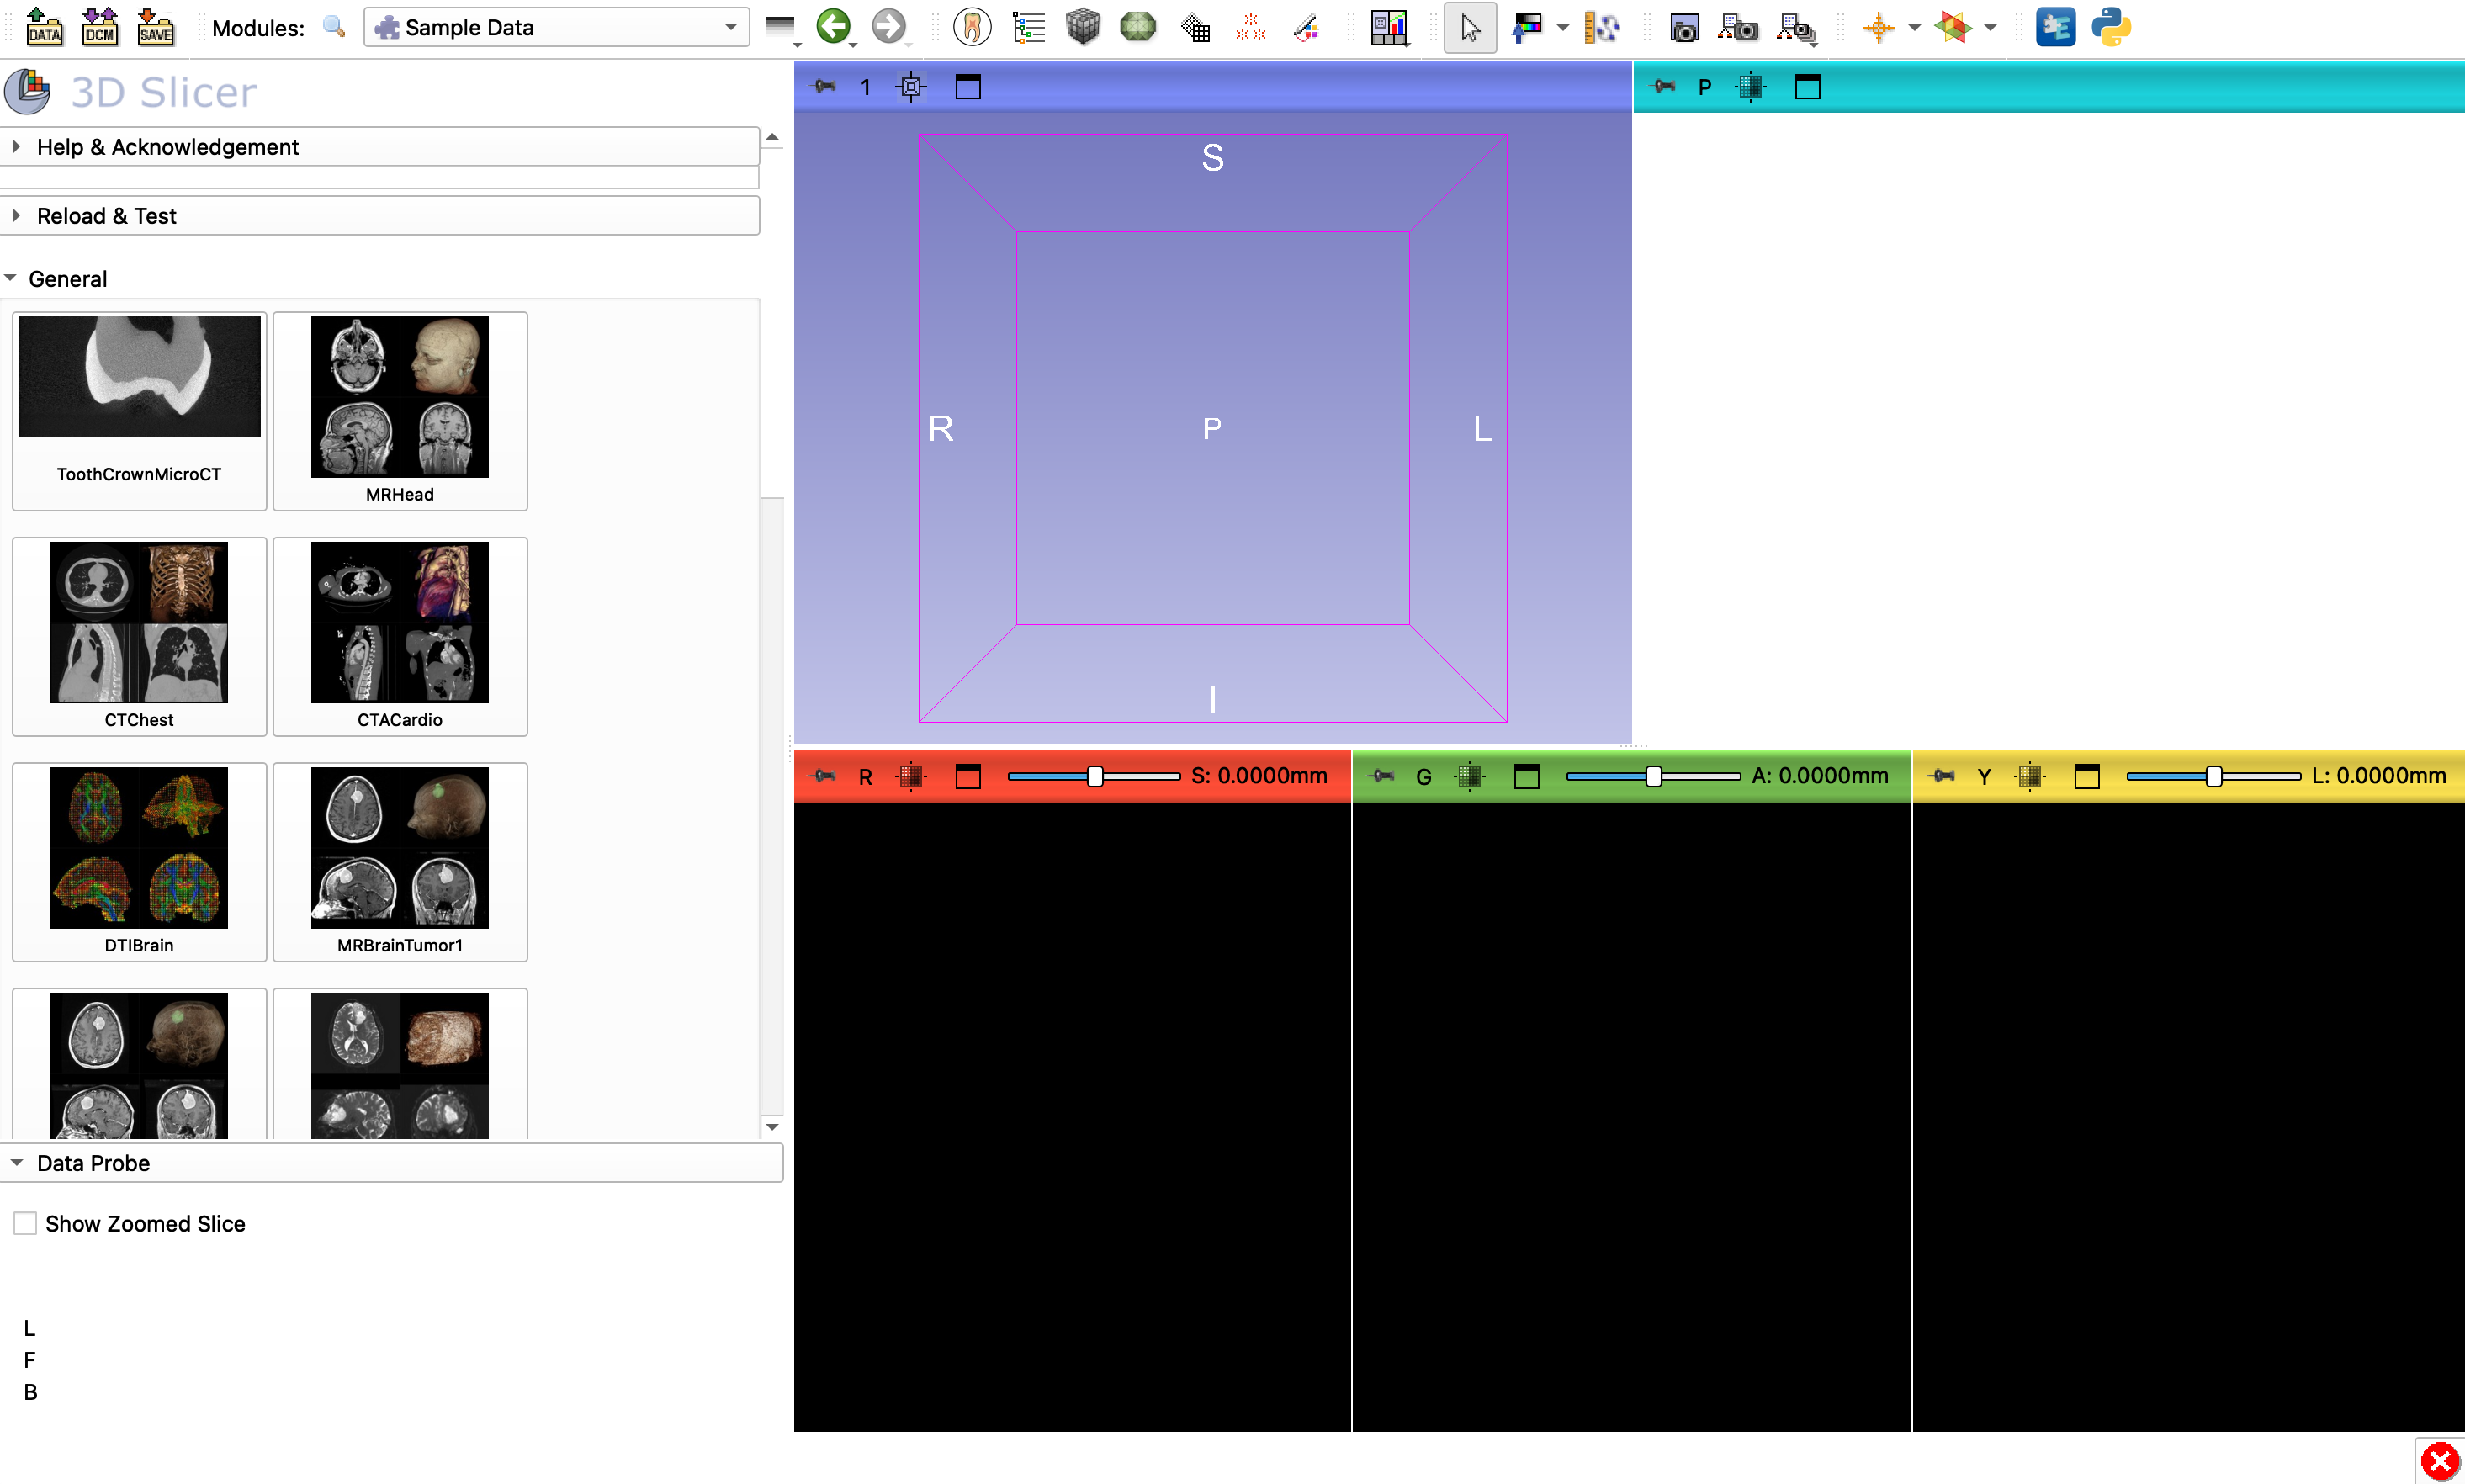
\includegraphics[width=1\textwidth]{img/sampleData.png}
	\caption{Ausschnitt des Moduls SampleData in 3D Slicer mit dem Beispielbild
	für das Starten eines Verfahrens im Tooth Analyser}
	\label{fig:sample_data}
\end{figure}

Ein Testfall der vielen soll hier Beispielhaft genauer betrachtet werden. Hierbei
geht es um den Test der Funktion \texttt{smoothImage()}. Diese Nimmt ein Bild und
führt eine Glättung durch. Um solch eine Funktion zu testen, bedarf es etwas mehr
als ein simplen Unittest, jedoch liefert der fertige Test eine gute Lösung um
den gesamten Umfang der Methode zu Testen. Vergleicht man ein verrauschtes Bild mit
einem geglätteten, dann unterschieden sie sich bis auf die visuelle Darstellung
auch in der Streuung der Pixelwerte. So kann mittels der Standardabweichung kontrolliert
werden, ob das Bild nach einer Filterung eine kleinere Standardabweichung hat
als vor der Filterung. Ist dies der Fall, so kann von einer erfolgreichen
Filterung ausgegangen werden. Zu Beachten ist an dieser Stelle, das eine
Filterung unter Umständen einige Zeit in Anspruch nehmen kann. Es sei gesagt,
dass diese bei einer Testausführung zu berücksichtigen ist. Eine gute Option dem
entgegenzuwirken ist es, das bereits gefilterte Bild mit in den Testdaten zur
Verfügung zu stellen. Die konkrete Implementierung eines solchen Tests liefert der
Quellcode \ref{lst:test_smooth_image}.

\begin{lstlisting}[
    language={python},
    caption={Implementierung eines Tests zum überprüfen einer Funktion},
    label={lst:test_smooth_image}]
def testSmoothImage(self):
    from ToothAnalyserLib.AnatomicalSegmentation.Segmentation import smoothImage
   
    data = self.getSampleDataAsITK()
    dataFiltered = smoothImage(data)
    dataStdDev = np.std(sitk.GetArrayFromImage(data))
    dataFilteredStdDev = np.std(sitk.GetArrayFromImage(dataFiltered))
    self.assertTrue(dataFilteredStdDev < dataStdDev)
    self.delayDisplay("Test 1 passed")
\end{lstlisting}

Im ersten Schritt wird ein Beispielbild geladen und in ein \ac{ITK} Format umgewandelt.
Anschließend folgt die Glättung des Bildes. Ist diese Glättung fertig, so können
die Streuungen der beiden Bilder verglichen werden.

Abschließend lässt sich über die Softwaretests sagen, dass einige Testfälle abgedeckt
wurden. Jedoch wurden nicht alle Methoden und Funktionen getestet. Viele bilden eine
sehr konkrete Lösung, die nicht einfach zu testen ist und deshalb einiges an
Entwicklungszeit beanspruchen. Gerade die Funktionen der Pipeline. Aus diesem
Grund konzentriert sich diese Arbeit nicht auf eine 100 prozentige Testabdeckung,
sondern soll noch weitere Metriken bieten. Eine ebenso gute Aussage lässt sich
anhand der Laufzeit des Moduls treffen. Hierzu wurde die Performance des Tooth Analyser
genauer unter die Lupe genommen und in verschiedenen Szenarien gemessen.

\pagebreak
% ---------------------------------------------------------------------------------------

\section{Performance}
Die Performance des Systems war nie ein wichtiges Kriterium und stand deshalb zu
keiner Zeit im Fokus dieser Arbeit. Dennoch ergaben sich interessante Ergebnisse,
die hier kurz erläutert werden sollen. Unter der Performance versteht dieses Kapitel
das konkrete Laufzeitverhalten der Anwendung also jene Zeit die zwischen Start und
Ende vergeht. Grundsätzlich lässt sich dazu sagen, dass die Laufzeit bei der Bearbeitung
von \ac{3D}-Mikro-\ac{CT}-Aufnahmen sehr stark vom Typ des Bildes abhängt. So kommt es
beispielsweise darauf an, wie groß das Bild ist, oder ob es bereits eine Filterung
erfahren hat. Bei der Verarbeitung der Mikro-\ac{CT}-Bilder aus dem Klinikum für
Zahnerhaltung wurde eine konkrete Messung durchgeführt, die hier in Abbildung
\ref{fig:laufzeit} gezeigt wird.

\textbf{Vorbedingungen:}
\begin{itemize}
	\item 16 bit sigend integer

	\item Type .ISQ

	\item Mit Filterung

	\item Mit Berechnung der medial Flächen
\end{itemize}

\begin{figure}[h]
	\centering
	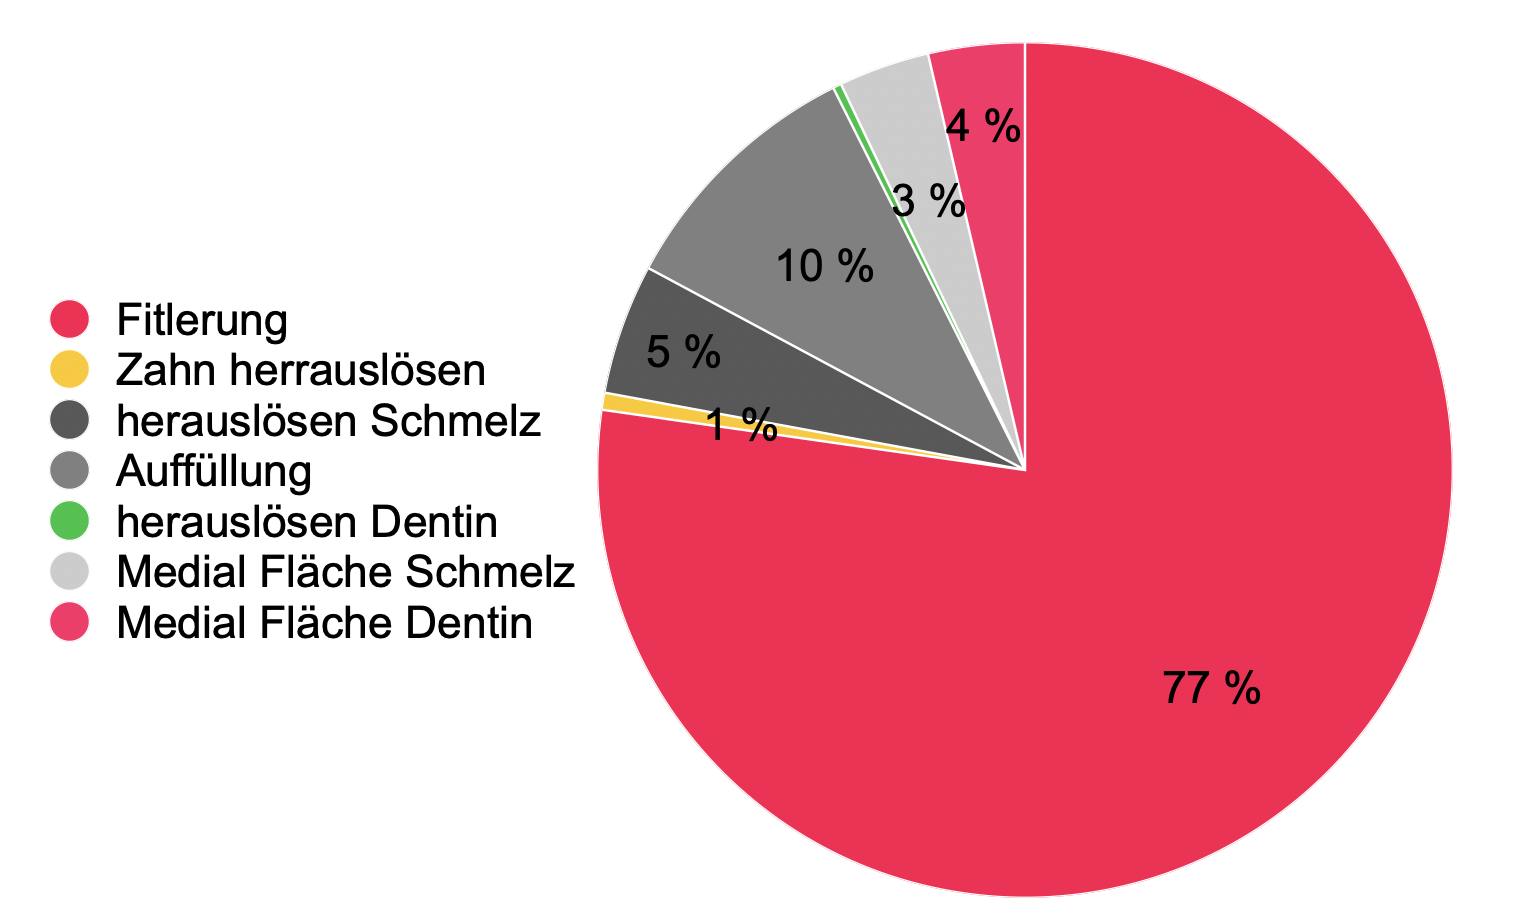
\includegraphics[width=0.8\textwidth]{img/laufzeit_diagramm.png}
	\caption{Verteilung der Laufzeit über den gesamten Bearbeitungszeitraum. 100\%
	entsprechen 16:27 Minuten}
	\label{fig:laufzeit}
\end{figure}

Zu sehen ist, dass unter diesen Bedingungen die Bearbeitung eines einzelnen
Bildes ca. 17 Minuten beansprucht. Dabei fallen über dreiviertel der Zeit auf
die Filterung zurück. Der Bereich Auffüllung beinhaltet ebenfalls eine Filterung
der einzelnen Segmente, weswegen dieser den zweitgrößten Teil ausmacht. Ein Weiterer
wesentlichen Teil stellen die beiden medialen Flächen dar. Um dieser doch
enormen Laufzeit etwas entgegen zu Wirken wurden zwei Mechanismen implementiert.
Das Verfahren kann einerseits erkennen, ob ein Bild bereits gefiltert wurde und
andererseits die medialen Flächen optional berechnen. So kommt es, dass sich ein
\textit{Best Case} ergibt der grob nur noch ein Viertel der Zeit benötigt.
Dieser \textit{Best Case} tritt ein, wenn ein Bild in den Algorithmus gegeben
wird, das bereits gefiltert wurde und keine medialen Flächen erfordert. Unter
Berücksichtigung von Abbildung \ref{fig:laufzeit} kann dann die Zeit für die
Filterung und die medialen Flächen abgezogen werden. So kommt es, dass das
Verfahren nur noch 16 Prozent der ursprünglichen Zeit benötigt.

Überträgt man das Laufzeitverhalten eines einzelnen Bildes auf die Bearbeitung
der Bilder in einem Batch-Prozess so lässt sich die Laufzeit mit der Anzahl der
zu bearbeitenden Bilder steigend linear ausdrücken. Das Diagramm aus \ref{fig:laufzeit_batch}
zeigt dies.

\begin{figure}[h]
	\centering
	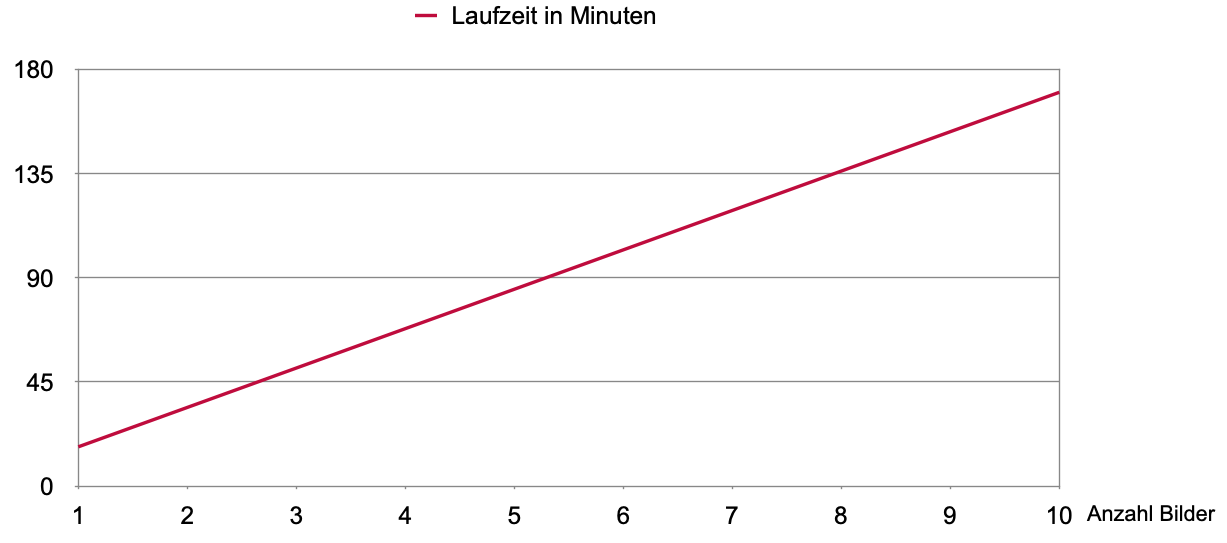
\includegraphics[width=1\textwidth]{img/runtimeBatch.png}
	\caption{Konstruktion des Laufzeitverhaltens bei einer Bearbeitung mehrere
	Bilder}
	\label{fig:laufzeit_batch}
\end{figure}

Wie zu sehen ist, ist die Laufzeit eines Batch Prozesses maßgeblich davon geprägt,
wie lange ein einzelnes Bild benötigt. Dies entspricht dem Y-Achsenabschnitt im Diagramm
\ref{fig:laufzeit_batch}. Ist die Zeit eines einzelnen Bildes bekannt, so lässt sich
gut prognostizieren, wie lange eine Verarbeitung von $n$ vielen Bildern dauert. Wie
bereits angedeutet, hängt die Zeit eines einzelnen Bilds von vielen Faktoren ab.
Nimmt man den Fall aus Abbildung \ref{fig:laufzeit}, würde die Bearbeitung von
zehn Bilder etwa 170 Minuten beanspruchen. Dies entspricht zwei Stunden und 50 Minuten.
% ---------------------------------------------------------------------------------------

\section{Benutzertests}
\label{sec:benutzertests}Um die entwickelte Software objektiv zu bewerten, wurden
gezielte Benutzertests mit Anwendern durchgeführt. Dabei nahmen drei Zahnärzte
der Poliklinik für Zahnerhaltung und Parodontologie an der LMU an der Testphase
teil, in der sie den Tooth Analyser in ihren Forschungsalltag integrierten. Über
einen Zeitraum von drei Wochen konnten sie die Software in realen
Anwendungsszenarien erproben.

Zusätzlich wurde ein kleiner Stresstest durchgeführt, bei dem 103 \ac{CT}-Aufnahmen in
einem Batch-Prozess mit dem Tooth Analyser verarbeitet wurden. Die Berechnung
erfolgte auf einem leistungsstarken Server der LMU, der über ausreichend Rechenkapazitäten
verfügt. Die durchschnittliche Bearbeitungszeit pro Bild lag hier bei etwa neun
Minuten. Basierend auf der in Abbildung \ref{fig:laufzeit_batch} dargestellten Verteilung
ergab sich eine prognostizierte Gesamtverarbeitungszeit von 15 Stunden und 27 Minuten.
Ein Wert, der in der Praxis gut bestätigt wurde. Besonders erfreulich war, dass sämtliche
Bilder bis zu einem gewissen Grad an Karies erfolgreich anatomisch segmentiert werden
konnten. Die Ergebnisse diese Batch-Prozesses sind dem Anhang zu entnehmen.
Die Tests in der Klinik zeigten zudem, dass auch die vollständige Segmentierung
ganzer Zähne mit komplexen Wurzeln möglich ist.

Die Ergebnisse der Benutzertests aus der Klinik verdeutlichen, dass der Tooth
Analyser in der Praxis eine wertvolle Unterstützung bietet, und durch die Segmentierung
ganzer Zähnen den Anwendungskreis noch weiter spannt. Um ein besseres
Verständnis für die realen Einsatzmöglichkeiten der Software zu gewinnen, werden
im folgenden Kapitel verschiedene Anwendungsszenarien vorgestellt.
% ---------------------------------------------------------------------------------------

\section{Anwendungsszenarien}
In erster Linie bietet der Tooth Analyser eine Visualisierungshilfe, die für
Ärzte unterstützend wirken soll. Wie auch von Slicer empfohlen wird dieses Modul
von den Ärzten rein zur Forschung eingesetzt. Mit dem Tooth Analyser lässt sich
mittels einer Mikro-\ac{CT}-Aufnahme ein \ac{3D}-Modell des Zahnes erstellen. Man
spricht hier von einer Rekonstruktion des Zahnes. Durch die Segmentierung erlaubt
dieser rekonstruierte Zahn auch eine Segmentbetrachtung von Dentin und Schmelz.
Die Abbildungen \ref{fig:3d_view}, \ref{fig:3d_view_dentin} und \ref{fig:3d_view_schmelz}
zeigt diese Rekonstruktion genauer.

\begin{figure}[h]
	\centering
	\begin{minipage}[b]{0.32\textwidth}
		\centering
		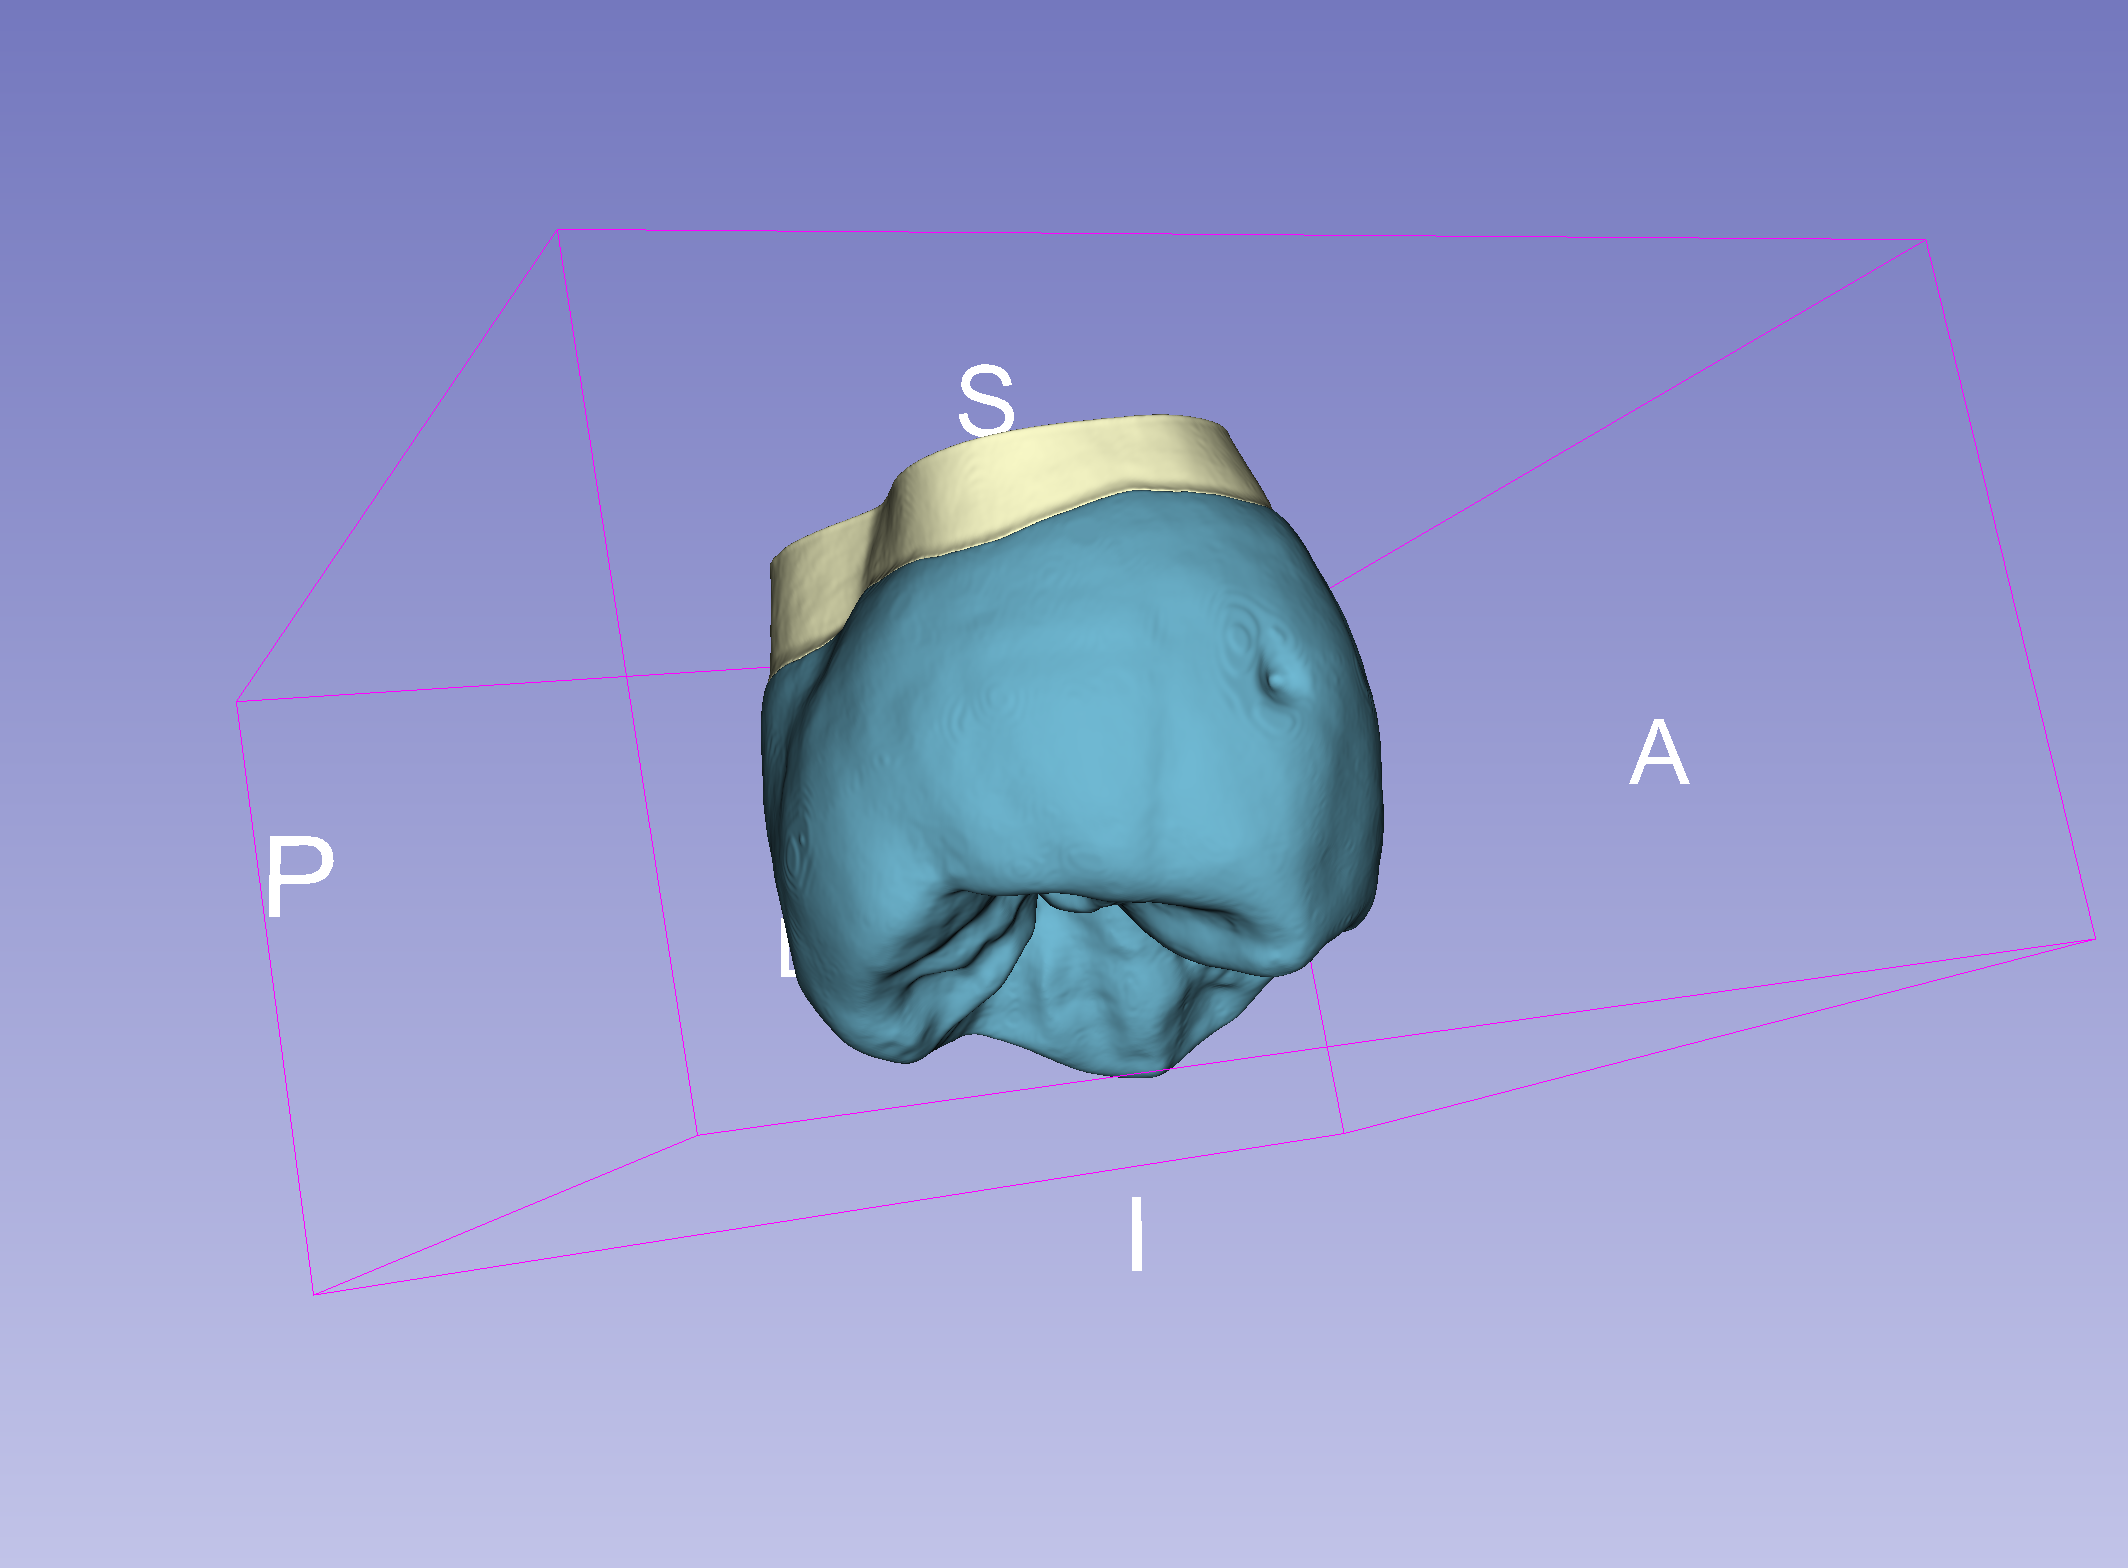
\includegraphics[width=\textwidth]{img/3dView.png}
		\caption{Rekonstruktion eines Zahns aus einer CT-Aufnahme}
		\label{fig:3d_view}
	\end{minipage}
	\hfill
	\begin{minipage}[b]{0.32\textwidth}
		\centering
		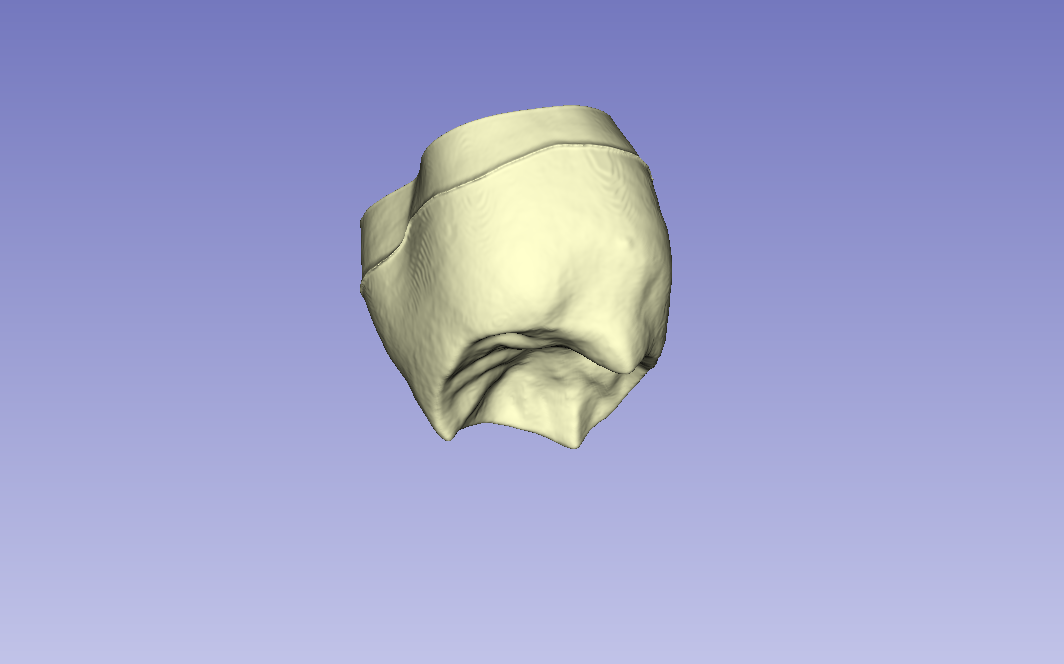
\includegraphics[width=\textwidth]{img/3dViewDentin.png}
		\caption{Dentinsegment eines rekonstruierten Zahns}
		\label{fig:3d_view_dentin}
	\end{minipage}
	\hfill
	\begin{minipage}[b]{0.32\textwidth}
		\centering
		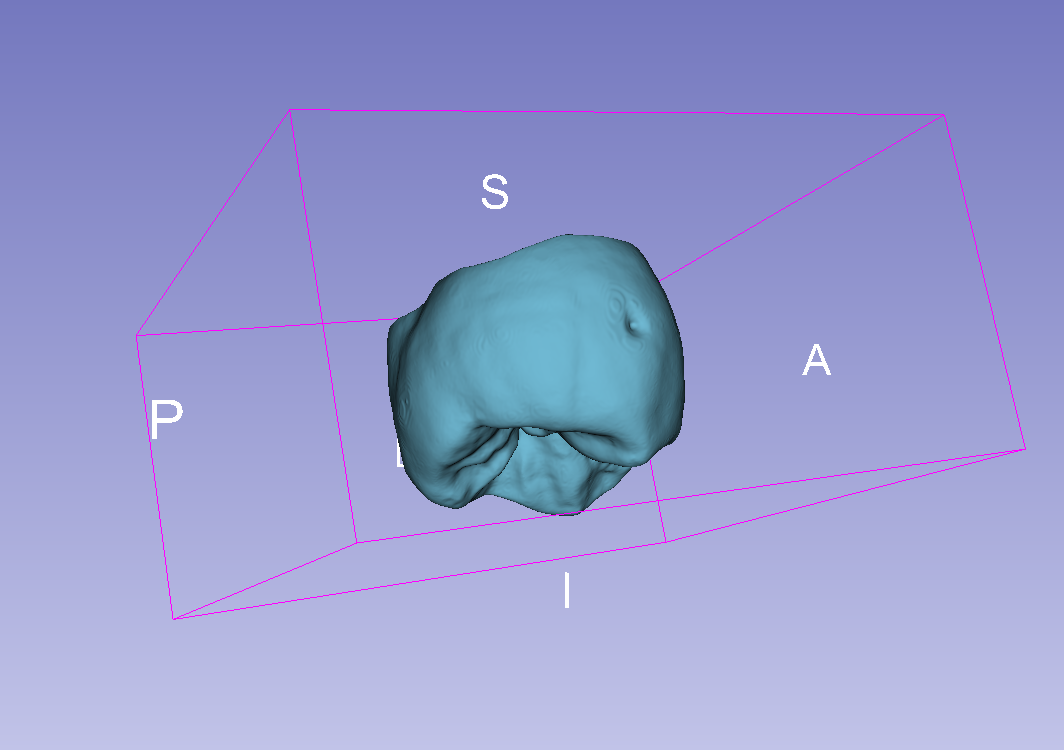
\includegraphics[width=\textwidth]{img/3dViewEnamel.png}
		\caption{Schmelzsegment eines rekonstruierten Zahns}
		\label{fig:3d_view_schmelz}
	\end{minipage}
\end{figure}

Das Betrachten der einzelnen Segmente wie sie in Abbildung
\ref{fig:3d_view_dentin} gezeigt wird, erfolgt nicht in der Erweiterung Tooth Analyser.
Hierzu wird auf das Modul \textit{Data} verwiesen, das eine hierarchische
Darstellung aller Daten in der Szene liefert. Über die Sichtbarkeitseinstellungen
der einzelnen Datenelemente können dann die Segmente sichtbar oder unsichtbar geschaltet
werden.

Einen weiteren Fall, indem die Anwendung unterstützen kann, ist die Klassifizierung
von Karies. Die Abbildung \ref{fig:classification} zeigt diesen Fall. Hierfür sind
die medialen Flächen der einzelnen Segmente nötig. Diese sind im Bild als rote
und grüne Linie sichtbar, verteilen sich aber über das ganze \ac{3D}-Bild, was daraus
eine Fläche macht. Legt man nun diese Flächen über das originale Bild, so lässt
sich mittels dieser Linie der Karies auf einem \ac{CT} gut klassifizieren. Diese
besagten Linien bilden dann die Grenzen. Ragt der Karies über diese mediale Fläche
hinaus hat er bereits einen sehr ausgeprägten Zustand und wird anders eingeordnet
als ein Karies, der die mediale Fläche noch nicht überschritten hat.

\begin{figure}[h]
	\centering
	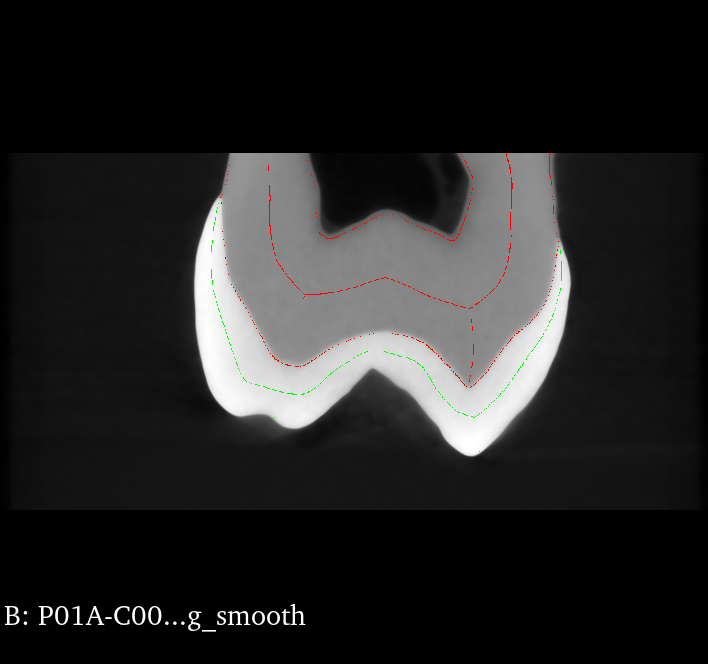
\includegraphics[width=0.4 \textwidth]{img/classification.png}
	\caption{Klassifizierung von Karies mittels der medialen Flächen}
	\label{fig:classification}
\end{figure}

Die konkreten Anwendungsfälle zeigen, dass der Tooth Analyser durchaus Anwendung
im Forschungsalltag der Klinik finden. Dennoch traten während der Nutzung auch einige
Einschränkungen auf, die die Einsatzmöglichkeiten des Tooth Analyser begrenzen.
% ---------------------------------------------------------------------------------------

\section{Limitierungen}
\label{sec:limitierungen} Dieses Kapitel soll alle Punkte transparent aufdecken,
die im Modul Tooth Analyser noch Probleme machen, oder gar nicht erst umgesetzt
wurden. Der limitierende Faktor in der Erweiterung ist das eingeschränkte Format
der Bilder. Es können innerhalb dieser Erweiterung nur Bilder verarbeitet werden,
die das Format \ac{16Int} haben. Führt man dennoch die Segmentierung mit einem anderen
Format durch (z.B. \ac{8UInt}), so stellt man fest, dass der Algorithmus zwar ein
Ergebnis generiert, dieses aber nicht verwendbar ist. Die Abbildung \ref{fig:3d_error}
zeigt ein solches falsche Ergebnis. Zu sehen ist ein \ac{3D}-Modell, das nur aus einem
Segment besteht. In diesem Fall wurde der gesamte Zahn mit Pulpa als Dentin
markiert.

\begin{figure}[h]
	\centering
	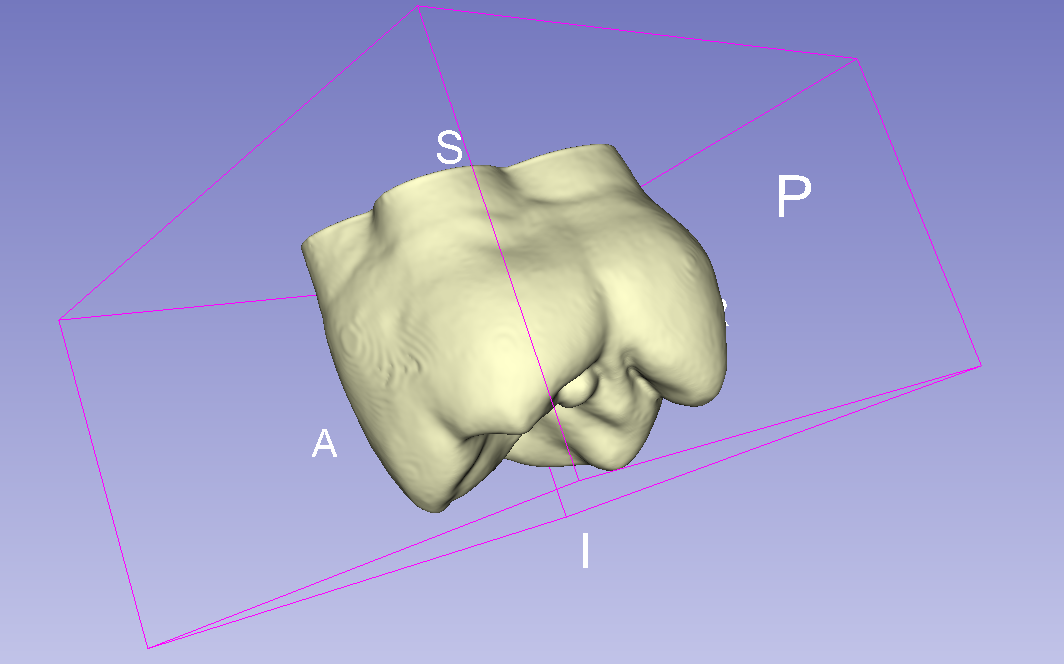
\includegraphics[width=0.5\textwidth]{img/3d_view_error.png}
	\caption{Fehlerhafte Segmentierung einer CT-Aufnahme im Format 8UInt}
	\label{fig:3d_error}
\end{figure}

Durch diese Limitierung ergibt sich eine weitere. Zu Beginn in der Analysephase
des Projektes, war eine Vorverarbeitung der Bilder vorgesehen, dass die
Komprimierung eines Bildes vornimmt und so die Bilder deutlich handlicher macht.
Das Verfahren hierzu wurde in Kapitel \ref{subsec:datensätze} erläutert. Da
dieses Verfahren allerdings einen Formatwechsel von \ac{16Int} nach \ac{8UInt}
bewirkt und diese Bilder nicht richtig segmentiert werden können, scheidet die Vorverarbeitung
von Bildern vorerst aus.

Eine weitere Limitierung liegt im Batch-Modus. Dieser steht laut der Struktur in
Kapitel \ref{sec:struktur_der_software} nicht nur für die ganze
Verarbeitungsvioline zur Verfügung, sondern auch für die einzelnen Schritte dieser
Pipeline. Da eine konkret implementierte Vorverarbeitung ohnehin vorerst
ausscheidet, wurde der Batch-Prozess nur für die reine anatomische Segmentierung
implementiert.

Zuletzt sei noch auf eine Limitierung hingewiesen, die der Erweiterbarkeit des
Moduls dient. Soll die Erweiterung um zusätzliche Funktionen erweiter werden,
dann sind kleine Änderungen in einer bestehenden Klasse notwendig. Konkret geht es
hier um die Klasse \texttt{ToothAnalyserWidget}. Hier muss je nach Ausprägung der
\ac{UI} der neuen Funktion, Methoden hinzugefügt werden.
% ---------------------------------------------------------------------------------------